\documentclass[a4paper,12pt]{article}

\usepackage{a4wide}
\usepackage{amsfonts}
\usepackage{amsmath}
\usepackage{amssymb}
\usepackage{lipsum}

\usepackage{graphicx}  % For including images

\usepackage{xcolor}  % For a colorfull presentation
\usepackage{listings}  % For presenting code 

\usepackage{hyperref}

% Definition of a style for code, matter of taste
\lstdefinestyle{mystyle}{
  language=Python,
  basicstyle=\ttfamily\footnotesize,
  backgroundcolor=\color[HTML]{F7F7F7},
  rulecolor=\color[HTML]{EEEEEE},
  identifierstyle=\color[HTML]{24292E},
  emphstyle=\color[HTML]{005CC5},
  keywordstyle=\color[HTML]{D73A49},
  commentstyle=\color[HTML]{6A737D},
  stringstyle=\color[HTML]{032F62},
  emph={@property,self,range,True,False},
  morekeywords={super,with,as,lambda},
  literate=%
    {+}{{{\color[HTML]{D73A49}+}}}1
    {-}{{{\color[HTML]{D73A49}-}}}1
    {*}{{{\color[HTML]{D73A49}*}}}1
    {/}{{{\color[HTML]{D73A49}/}}}1
    {=}{{{\color[HTML]{D73A49}=}}}1
    {/=}{{{\color[HTML]{D73A49}=}}}1,
  breakatwhitespace=false,
  breaklines=true,
  captionpos=b,
  keepspaces=true,
  numbers=none,
  showspaces=false,
  showstringspaces=false,
  showtabs=false,
  tabsize=4,
  frame=single,
}
\lstset{style=mystyle}

\begin{document}
\title{Machine Learning A (2024)\\Home Assignment 1}
\author{Carlo Rosso rkm957}
\date{}
\maketitle

% Please leave the table of contents as is, for the ease of navigation for TAs
\tableofcontents % Generates the table of contents
\newpage % Start a new page after the table of contents

\section{Make Your Own (10 points)}

I am going to follow the order of the question and I am going to answer them one
by one, follows the answers to the first question.

% Enumerator environment, add items as needed
\begin{enumerate}
	\item I would collect, the grade to each assignment, their grades' mean,
	      their study program and their attendance to the lectures. Let $n_a$ be
	      the number of assignments and $G$ the set of grades you can take in
	      each assignment (considering they can only be the same, for
	      semplicity), $S$ the set of study programs and let the attendance be
	      the ratio between attended class over the total number of class this
	      far. Then
	      $\mathcal{X} = G^{n_a} \times [2, 12] \times S \times [0, 1]$.

	\item The label space $\mathcal{Y}$ is the set of all possible grades that
	      can be taken in the final exam, so $\mathcal{Y} = G$ (referring to the
	      previous question).

	\item I would define the lost function as the mean squared error between the
	      predicted grade and the real grade, so $\mathcal{l}(y', y) = (y' -
		      y)^2$.

	\item I define the distance measure as the absolute difference
	      ($|x_1 - x_2|$) in each
	      dimension which already defines such an operation and I would use the
	      following formula for the computation of the distance in the $S$
	      dimension:
	      \begin{equation}
		      d(s_1, s_2) = \begin{cases}
			      0 & \text{if } s_1 = s_2 \\
			      1 & \text{otherwise}.
		      \end{cases}
	      \end{equation}

	\item I think it is a quite basic algorithm, so I suppose it would obtain
	      some kind of result, but I am not able to guess any result, I don't
	      think I am very good at guessing. I think it can be considered a good
	      starting point for the model, but I also think you should try many
	      different lost functions and distance measures to see which one works
	      the best.

	\item There could be privacy issue on how you get access to the
	      information to build the model. Data can be too sparse or too noisy.
\end{enumerate}

\section{Digits Classification with $K$ Nearest Neighbors (40 points)}

\subsection{Task \#1}

% Placeholder code
\begin{lstlisting}
def distance(x, y):
    return np.sum((x - y) ** 2)

def compute_predictions(distances, training_labels):
  sorted_distances = np.argsort(distances)
  predictions = np.cumsum(training_labels[sorted_distances])
  return [-1 if x < 0 else 1 for x in predictions]

def loss(predictions, labels):
  return np.sum((labels != predictions)) / len(predictions)

def knn(training_data, training_labels, test_data, test_labels):
  distances = [[distance(x, x_train) for x_train in training_data] for x in test_data]
  predictions = np.array([compute_predictions(x, training_labels) for x in distances]).T
  return [loss(x, test_labels) for x in predictions]
\end{lstlisting}

% Placeholder figure
\begin{figure}[htbp]
	\centering
	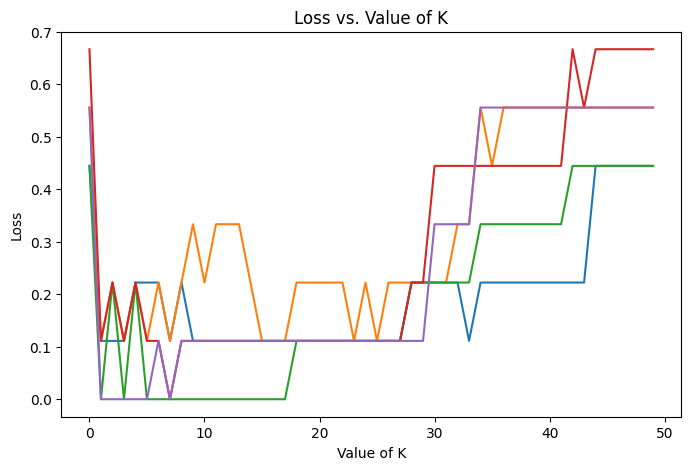
\includegraphics[width=0.5\textwidth]{1}
	\caption{Validation test of size 10: influence of k over the loss}
\end{figure}

\begin{figure}[htbp]
	\centering
	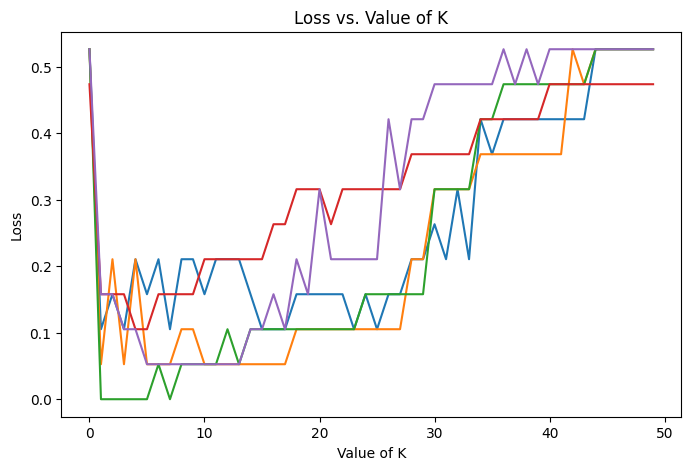
\includegraphics[width=0.5\textwidth]{2}
	\caption{Validation test of size 20: influence of k over the loss}
\end{figure}

\begin{figure}[htbp]
	\centering
	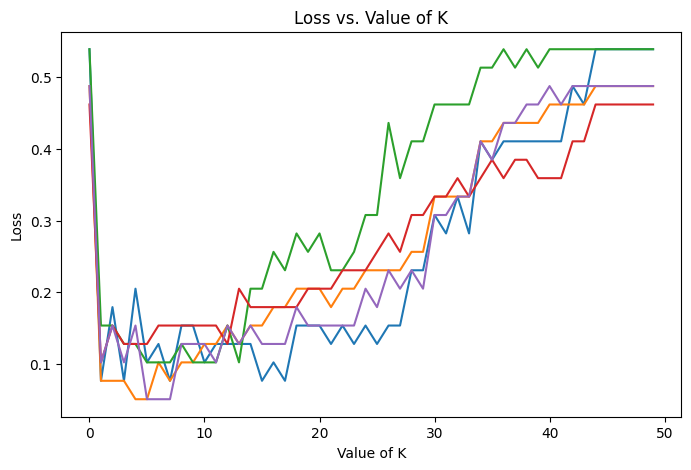
\includegraphics[width=0.5\textwidth]{3}
	\caption{Validation test of size 40: influence of k over the loss}
\end{figure}

\begin{figure}[htbp]
	\centering
	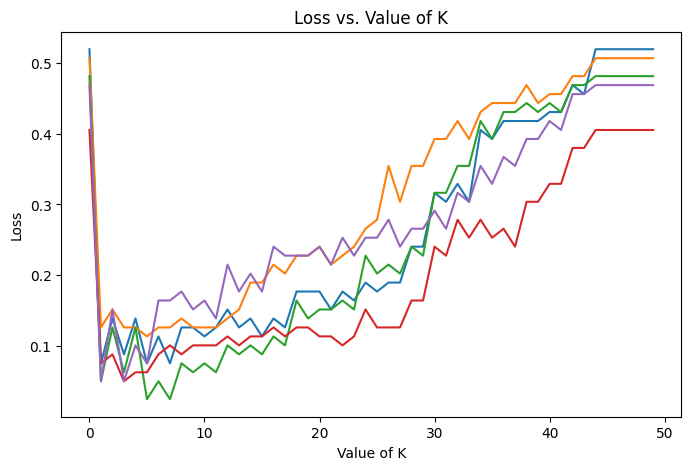
\includegraphics[width=0.5\textwidth]{4}
	\caption{Validation test of size 80: influence of k over the loss}
\end{figure}

\begin{figure}[htbp]
	\centering
	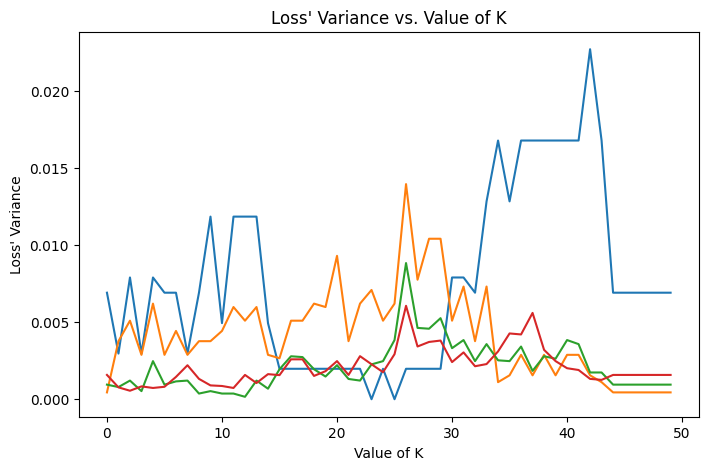
\includegraphics[width=0.5\textwidth]{5}
	\caption{Influence of k over validation errors' variance}
\end{figure}

\subsubsection{What can you say about fluctuations of the validation error as a
	function of $n$?}

The fluctuations of the validation error seems to decrease with the number of
samples in the test set. This is probably due to the fact that the more samples
you have, the more precise we compute the loss.

\subsubsection{What can you say about the prediction accuracy of K-NN as a
	function of K?}

It looks like it doesn't really matter the size of the test set, the accuracy is
going to be at the highest as long as $1 < k < 15$, then it starts to decrease.
In addition, I suppose it decreases linearly with $k$ up to $k = 50$, since that is
the maximum value of $k$ we have tested. When $k = 50$ the accuracy gets to be
about 50\%. Noting that this is a binary classification problem, the algorithm
at $k = 50$ is as good as a random guess.

\bibliography{bibliography}  % If you have some references, use BibTeX

\end{document}
